%%%%%%%%%%%%%%%%%%%%%%%%%%%%%%%%%%%%%%%%%
% Masters/Doctoral Thesis 
% LaTeX Template
% Version 2.5 (27/8/17)
%
% This template was downloaded from:
% http://www.LaTeXTemplates.com
%
% Version 2.x major modifications by:
% Vel (vel@latextemplates.com)
%
% This template is based on a template by:
% Steve Gunn (http://users.ecs.soton.ac.uk/srg/softwaretools/document/templates/)
% Sunil Patel (http://www.sunilpatel.co.uk/thesis-template/)
%
% Template license:
% CC BY-NC-SA 3.0 (http://creativecommons.org/licenses/by-nc-sa/3.0/)
%
%%%%%%%%%%%%%%%%%%%%%%%%%%%%%%%%%%%%%%%%%

%----------------------------------------------------------------------------------------
%	PACKAGES AND OTHER DOCUMENT CONFIGURATIONS
%----------------------------------------------------------------------------------------

\documentclass[
11pt, % The default document font size, options: 10pt, 11pt, 12pt
oneside, % Two side (alternating margins) for binding by default, uncomment to switch to one side
english, % ngerman for German
singlespacing, % Single line spacing, alternatives: onehalfspacing or doublespacing
%draft, % Uncomment to enable draft mode (no pictures, no links, overfull hboxes indicated)
%nolistspacing, % If the document is onehalfspacing or doublespacing, uncomment this to set spacing in lists to single
%liststotoc, % Uncomment to add the list of figures/tables/etc to the table of contents
%toctotoc, % Uncomment to add the main table of contents to the table of contents
%parskip, % Uncomment to add space between paragraphs
%nohyperref, % Uncomment to not load the hyperref package
headsepline, % Uncomment to get a line under the header
%chapterinoneline, % Uncomment to place the chapter title next to the number on one line
%consistentlayout, % Uncomment to change the layout of the declaration, abstract and acknowledgements pages to match the default layout
]{MastersDoctoralThesis} % The class file specifying the document structure

\usepackage[utf8]{inputenc} % Required for inputting international characters
\usepackage[T1]{fontenc} % Output font encoding for international characters

\usepackage{mathpazo} % Use the Palatino font by default

\usepackage[backend=bibtex,style=authoryear,natbib=true, sorting=none]{biblatex} % Use the bibtex backend with the authoryear citation style (which resembles APA)

\addbibresource{references.bib} % The filename of the bibliography

\usepackage[autostyle=true]{csquotes} % Required to generate language-dependent quotes in the bibliography

\usepackage{listings}

\usepackage{tabularx} % Uncomment to allow columns to automatically adjust to the page width
%----------------------------------------------------------------------------------------
%	MARGIN SETTINGS
%----------------------------------------------------------------------------------------

\geometry{
	paper=a4paper, % Change to letterpaper for US letter
	inner=2.5cm, % Inner margin
	outer=3.8cm, % Outer margin
	bindingoffset=.5cm, % Binding offset
	top=1.5cm, % Top margin
	bottom=1.5cm, % Bottom margin
	%showframe, % Uncomment to show how the type block is set on the page
}

%----------------------------------------------------------------------------------------
%	THESIS INFORMATION
%----------------------------------------------------------------------------------------

\thesistitle{Development of a Virtual interactive Laboratory Testbench for Socially-Aware Robot Navigation} % Your thesis title, this is used in the title and abstract, print it elsewhere with \ttitle
\supervisor{Prof. Dr.-Ing Stefan Friedrich} % Your supervisor's name, this is used in the title page, print it elsewhere with \supname
\examiner{Prof. Dr. Rainer Herrler} % Your examiner's name, this is not currently used anywhere in the template, print it elsewhere with \examname
\degree{B.Eng. Mechatronics } % Your degree name, this is used in the title page and abstract, print it elsewhere with \degreename
\author{Prince Sakariya} % Your name, this is used in the title page and abstract, print it elsewhere with \authorname
\addresses{} % Your address, this is not currently used anywhere in the template, print it elsewhere with \addressname

\subject{Biological Sciences} % Your subject area, this is not currently used anywhere in the template, print it elsewhere with \subjectname
\keywords{} % Keywords for your thesis, this is not currently used anywhere in the template, print it elsewhere with \keywordnames
\university{\href{https://www.thws.de/}{Technische Hochschule Würzburg-Schweinfurt}} % Your university's name and URL, this is used in the title page and abstract, print it elsewhere with \univname
\department{\href{http://department.university.com}{Department or School Name}} % Your department's name and URL, this is used in the title page and abstract, print it elsewhere with \deptname
\group{\href{http://researchgroup.university.com}{Research Group Name}} % Your research group's name and URL, this is used in the title page, print it elsewhere with \groupname
\faculty{\href{https://fe.thws.de/}{Faculty of Electrical and Mechanical Engineering}} % Your faculty's name and URL, this is used in the title page and abstract, print it elsewhere with \facname

\AtBeginDocument{
\hypersetup{pdftitle=\ttitle} % Set the PDF's title to your title
\hypersetup{pdfauthor=\authorname} % Set the PDF's author to your name
\hypersetup{pdfkeywords=\keywordnames} % Set the PDF's keywords to your keywords
}

\begin{document}

\frontmatter % Use roman page numbering style (i, ii, iii, iv...) for the pre-content pages

\pagestyle{plain} % Default to the plain heading style until the thesis style is called for the body content

%----------------------------------------------------------------------------------------
%	TITLE PAGE
%----------------------------------------------------------------------------------------

\begin{titlepage}
\begin{center}

\vspace*{.06\textheight}
{\scshape\LARGE \univname\par}\vspace{1.5cm} % University name
\textsc{\Large Bachelor Thesis}\\[0.5cm] % Thesis type

\HRule \\[0.4cm] % Horizontal line
{\huge \bfseries \ttitle\par}\vspace{0.4cm} % Thesis title
\HRule \\[1.5cm] % Horizontal line
 
\begin{minipage}[t]{0.4\textwidth}
\begin{flushleft} \large
\emph{Author:}\\
\href{https://prince-sakariya.github.io/Prince-Sakariya/}{\authorname} % Author name - remove the \href bracket to remove the link
\end{flushleft}
\end{minipage}
\begin{minipage}[t]{0.4\textwidth}
\begin{flushright} \large
\emph{Supervisor:} \\
\href{https://fe.thws.de/projekt-und-forschungsmaster-met/fakultaet/personen/professorenkollegium/?tx_fhwspersonen_fe%5Bperson%5D=4042&tx_fhwspersonen_fe%5Bcontroller%5D=Person&cHash=772003982e695edfaf9d5e65b85d3d53}{\supname} % Supervisor name - remove the \href bracket to remove the link  
\end{flushright}
\end{minipage}\\[3cm]
 
\vfill

\large \textit{A thesis submitted in fulfillment of the requirements\\ for the degree of \degreename}\\[0.3cm] % University requirement text
% \textit{in the}\\[0.4cm]
% \groupname\\\deptname\\[2cm] % Research group name and department name
 
\vfill

{\large \today}\\[4cm] % Date

\includegraphics[scale=0.1]{Figures/Logo} % University/department logo - uncomment to place it
 
\vfill
\end{center}
\end{titlepage}

%----------------------------------------------------------------------------------------
%	DECLARATION PAGE
%----------------------------------------------------------------------------------------

\begin{declaration}
\addchaptertocentry{\authorshipname} % Add the declaration to the table of contents
\noindent I, \authorname, declare that this thesis titled, \enquote{\ttitle} and the work presented in it are my own. I confirm that:

\begin{itemize} 
\item This work was done wholly or mainly while in candidature for a research degree at this University.
\item Where any part of this thesis has previously been submitted for a degree or any other qualification at this University or any other institution, this has been clearly stated.
\item Where I have consulted the published work of others, this is always clearly attributed.
\item Where I have quoted from the work of others, the source is always given. With the exception of such quotations, this thesis is entirely my own work.
\item I have acknowledged all main sources of help.
\item Where the thesis is based on work done by myself jointly with others, I have made clear exactly what was done by others and what I have contributed myself.\\
\end{itemize}
 
\noindent Signed:\\
\rule[0.5em]{25em}{0.5pt} % This prints a line for the signature
 
\noindent Date:\\
\rule[0.5em]{25em}{0.5pt} % This prints a line to write the date
\end{declaration}

\cleardoublepage

%----------------------------------------------------------------------------------------
%	QUOTATION PAGE
%----------------------------------------------------------------------------------------

% \vspace*{0.2\textheight}

% \noindent\enquote{\itshape Thanks to my solid academic training, today I can write hundreds of words on virtually any topic without possessing a shred of information, which is how I got a good job in journalism.}\bigbreak

% \hfill Dave Barry

%----------------------------------------------------------------------------------------
%	ABSTRACT PAGE
%----------------------------------------------------------------------------------------

\begin{abstract}
\addchaptertocentry{\abstractname} % Add the abstract to the table of contents
The Thesis Abstract is written here (and usually kept to just this page). The page is kept centered vertically so can expand into the blank space above the title too\ldots
\end{abstract}

%----------------------------------------------------------------------------------------
%	ACKNOWLEDGEMENTS
%----------------------------------------------------------------------------------------

\begin{acknowledgements}
\addchaptertocentry{\acknowledgementname} % Add the acknowledgements to the table of contents
The acknowledgments and the people to thank go here, don't forget to include your project advisor\ldots
\end{acknowledgements}

%----------------------------------------------------------------------------------------
%	LIST OF CONTENTS/FIGURES/TABLES PAGES
%----------------------------------------------------------------------------------------

\tableofcontents % Prints the main table of contents

\listoffigures % Prints the list of figures

\listoftables % Prints the list of tables

%----------------------------------------------------------------------------------------
%	ABBREVIATIONS
%----------------------------------------------------------------------------------------

% \begin{abbreviations}{ll} % Include a list of abbreviations (a table of two columns)

% \textbf{LAH} & \textbf{L}ist \textbf{A}bbreviations \textbf{H}ere\\
% \textbf{WSF} & \textbf{W}hat (it) \textbf{S}tands \textbf{F}or\\

% \end{abbreviations}

%----------------------------------------------------------------------------------------
%	PHYSICAL CONSTANTS/OTHER DEFINITIONS
%----------------------------------------------------------------------------------------

% \begin{constants}{lr@{${}={}$}l} % The list of physical constants is a three column table

% % The \SI{}{} command is provided by the siunitx package, see its documentation for instructions on how to use it

% Speed of Light & $c_{0}$ & \SI{2.99792458e8}{\meter\per\second} (exact)\\
% %Constant Name & $Symbol$ & $Constant Value$ with units\\

% \end{constants}

%----------------------------------------------------------------------------------------
%	SYMBOLS
%----------------------------------------------------------------------------------------

% \begin{symbols}{lll} % Include a list of Symbols (a three column table)

% $a$ & distance & \si{\meter} \\
% $P$ & power & \si{\watt} (\si{\joule\per\second}) \\
% %Symbol & Name & Unit \\

% \addlinespace % Gap to separate the Roman symbols from the Greek

% $\omega$ & angular frequency & \si{\radian} \\

% \end{symbols}

%----------------------------------------------------------------------------------------
%	DEDICATION
%----------------------------------------------------------------------------------------

% \dedicatory{For/Dedicated to/To my\ldots} 

%----------------------------------------------------------------------------------------
%	THESIS CONTENT - CHAPTERS
%----------------------------------------------------------------------------------------

\mainmatter % Begin numeric (1,2,3...) page numbering

\pagestyle{thesis} % Return the page headers back to the "thesis" style

% Include the chapters of the thesis as separate files from the Chapters folder
% Uncomment the lines as you write the chapters

% Chapter Template

\chapter{Introduction} % Main chapter title

\label{Chapter1} % Change X to a consecutive number; for referencing this chapter elsewhere, use \ref{ChapterX}

%----------------------------------------------------------------------------------------
%	SECTION 1
%----------------------------------------------------------------------------------------

\section{Background and Motivation}
% Robot navigation in human environments requires more than obstacle avoidance;
% it demands social awareness and adherence to human proxemic norms. While 
% traditional navigation focuses on collision avoidance and path optimization, 
% social navigation must account for human comfort, cultural norms, and implicit 
% social rules. Socially-aware robot interaction is a very complex topic and 
% interdisciplinary by design. It covers robot navigation tasks, social and 
% cultural rules as well as Human Behaviour Analysis \cite{MOLLERsurvey}. 
% The development of such mobile social robots poses two main challenges: first, 
% real experimentation with people is costly and can be dangerous mainly during
% the initial stages of development, second, difficult to perform and to replicate
% except for very limited, controlled scenarios. Recent years have seen strides in 
% social robotics \cite{arenarosnav}, \cite{hunavsimros2human}, \cite{habitat} 
% with numerous research works proposing platforms and approaches for social 
% navigation and benchmarking. 

As robots increasingly operate in human-populated environments such as hospitals, 
shopping malls, and homes, traditional navigation approaches focused solely on 
collision avoidance and path optimization have proven insufficient. 
Socially-aware navigation represents a critical advancement that extends 
beyond obstacle avoidance to incorporate human comfort, cultural norms, 
and implicit social conventions. This evolution is essential for robots to gain 
acceptance in shared human spaces.
Social navigation is inherently interdisciplinary, bridging robotics, social 
psychology, cultural anthropology, and human-computer interaction. At its core 
lies the concept of proxemics—the study of human use of space and its cultural 
variations—first introduced by anthropologist Edward T. Hall in 1966. Hall's 
delineation of intimate, personal, social, and public interaction zones provides 
a fundamental framework for robot navigation in human environments, as respecting 
these invisible boundaries is crucial for social acceptance.
The development of socially-aware mobile robots faces several significant challenges:
\begin{itemize}
    \item \textit{Complexity of Social Rules} - Human spatial behavior is governed by implicit, 
    context-dependent rules that vary across cultures and situations. These rules are 
    typically learned intuitively by humans but must be explicitly encoded for robots.
    \item \textit{Experimentation Challenges} - Real-world testing with humans is 
    resource-intensive, potentially risky during early development stages, and 
    difficult to reproduce consistently across different research groups.
    \item \textit{Interdisciplinary Knowledge Requirements} - Developing effective social navigation 
    systems demands expertise across multiple domains, creating both research and 
    educational barriers.
    \item \textit{Technical Implementation Hurdles} - Integrating social awareness into existing 
    navigation frameworks requires sophisticated software architecture and computational 
    efficiency to maintain real-time performance.
\end{itemize}

Recent advances in social robotics have produced numerous platforms and approaches for 
addressing these challenges (\cite{arenarosnav}, \cite{hunavsimros2human}, \cite{habitat}). 
However, these innovations often remain siloed within research laboratories, with limited 
accessibility for educational purposes. This accessibility gap represents a significant 
obstacle for preparing the next generation of roboticists to develop socially-aware systems.
%----------------------------------------------------------------------------------------
%	SECTION 2
%----------------------------------------------------------------------------------------

\section{Problem Statement}
Often times, navigation systems treat humans as mere dynamic obstacles without 
considering social contexts, leading to behaviors that may be technically efficient 
but socially inappropriate. This research addresses the gap between technically 
sound and socially acceptable robot navigation in human-shared spaces. 

Despite significant research advances in social navigation, three critical problems persist:
\begin{enumerate}
    \item \textit{Technical-Social Disconnect} - Most deployed robot navigation systems continue to treat 
    humans as mere dynamic obstacles, disregarding social contexts and norms. This approach 
    leads to behaviors that may be computationally efficient but socially inappropriate or 
    discomforting to humans sharing the space.
    \item \textit{Educational Access Barriers} - Existing social navigation implementations typically demand 
    extensive technical expertise and computational resources, making them inaccessible for 
    educational purposes. Students face significant hurdles in learning about and 
    experimenting with social navigation concepts due to complex installation requirements, 
    dependencies, and hardware constraints.
    \item \textit{Lack of Standardized Learning Tools} - While several research platforms exist, there is a 
    notable absence of standardized educational tools that demonstrate social navigation 
    concepts in a structured, pedagogically sound manner. This gap impedes effective 
    teaching and learning of this increasingly important aspect of robotics.
\end{enumerate}

This thesis addresses these interconnected problems by developing an accessible, education-focused platform that bridges the gap between advanced social navigation research and practical robotics education.
%----------------------------------------------------------------------------------------
%	SECTION 3
%----------------------------------------------------------------------------------------

\section{Research objectives}
% As part of the Bachelor thesis, the system will be developed with educational use in mind.
% The goal is to create a testbench for social robot navigation that allows to be employed 
% both reserach and teaching purposes: a virtual laboratory experiment that a) demonstrate 
% a variety of off-the-shelf social navigation algorithms, b) show the effect of user-defined
% custom cost functions and/or evaluation metrics used in navigation algorithms, c) modify 
% human behaviour simulation, and (optionally / ideally) d) run custom social navigation 
% algorithms. The following subsections define the tasks in detail.

This bachelor thesis aims to develop an educational system for teaching and experimenting 
with social robot navigation concepts. The primary goal is to create a virtual laboratory 
environment that lowers technical barriers and provides structured learning experiences. 
Specific objectives include:

\begin{enumerate}
    \item \textbf{Create an accessible virtual testbench} that demonstrates various social navigation concepts 
    without requiring extensive technical setup or specialized hardware. This environment will:
    \begin{itemize}
        \item Integrate existing open-source social navigation implementations
        \item Provide a virtualized environment that runs efficiently on standard student hardware
        \item Offer a unified interface for interaction with different navigation approaches
    \end{itemize}
    
    \item \textbf{Develop structured educational experiments} that:
    \begin{itemize}
        \item Demonstrate a variety of off-the-shelf social navigation algorithms
        \item Illustrate the effects of different proxemic models and parameter configurations
        \item Allow comparison between socially-aware and traditional navigation approaches
        \item Showcase the impact of environmental context on navigation behavior
    \end{itemize}
    
    \item \textbf{Enable hands-on experimentation} through:
    \begin{itemize}
        \item Real-time costmap parameter modification
        \item Customizable evaluation metrics for navigation performance
        \item Visualization tools for understanding algorithm decision-making
    \end{itemize}
    
    \item \textbf{Create comprehensive educational materials} including:
    \begin{itemize}
        \item Laboratory exercises with clear learning objectives
        \item Documentation explaining theoretical concepts and their implementation
        \item Guided exploration activities with progressive complexity
    \end{itemize}
\end{enumerate}


The system is designed primarily for undergraduate and graduate robotics courses, 
enabling students to develop an intuitive understanding of social navigation 
principles through direct experimentation before potentially developing their 
own implementations.
%----------------------------------------------------------------------------------------
%	SECTION 4
%----------------------------------------------------------------------------------------

\section{Scope and Limitations}

This thesis focuses on creating an educational platform for social navigation rather than developing novel navigation algorithms or proxemic models. The scope encompasses:

\subsection*{In Scope:}
\begin{itemize}
    \item Integration of existing open-source social navigation implementations
    \item Development of a virtualized environment for accessible deployment
    \item Creation of standardized test scenarios for comparative evaluation
    \item Design of structured educational experiments and supporting materials
    \item Implementation of visualization tools for algorithm behavior and decision processes
    \item Extension of existing platforms with missing components required for educational purposes
\end{itemize}

\subsection*{Out of Scope:}
\begin{itemize}
    \item Development of fundamentally new social navigation algorithms
    \item Large-scale human studies to validate navigation approaches
    \item Physical robot implementation and testing
    \item Cross-platform compatibility beyond the specified virtualization approach
    \item Comprehensive cultural adaptation of proxemic models
\end{itemize}

\subsection*{Limitations:}
\begin{itemize}
    \item The system will prioritize educational clarity over computational performance
    \item Simulated human behaviors will represent simplified models of actual human movement patterns
    \item The virtualized environment introduces some performance overhead compared to native installation
    \item The platform targets educational use cases rather than deployment-ready implementations
\end{itemize}

These scope boundaries ensure the project remains achievable within the constraints of a 
bachelor thesis while still delivering significant educational value through an accessible 
platform for teaching social navigation concepts.
% Chapter Template

\chapter{Literature Review} % Main chapter title

\label{Chapter2} % Change X to a consecutive number; for referencing this chapter elsewhere, use \ref{ChapterX}

%----------------------------------------------------------------------------------------
%	SECTION 1
%----------------------------------------------------------------------------------------

\section{Social Navigation in Robotics}

%-----------------------------------
%	SUBSECTION 1
%-----------------------------------
\subsection{Definition and Importance}
\cite{riosmartinez2015proxemics}\ gave a compact description of socially-aware navigation: 
\emph{``Socially-aware navigation is the strategy exhibited by a social robot that identifies 
and follows social conventions (in terms of management of space) to preserve a comfortable 
interaction with humans. The resulting behavior is predictable, adaptable, and easily 
understood by humans.''} This definition implies that, from the robot's point of view, 
humans are no longer perceived only as dynamic obstacles but also as social entities.

The importance of social navigation is paramount for robots (\cite{KRUSE20131726}) intended to operate in human-centric 
environments such as homes, hospitals, shopping malls, offices, and public spaces. 
As robots become increasingly integrated into our daily lives, their ability to interact seamlessly 
and naturally with humans is crucial for their acceptance and widespread adoption. Poor social 
navigation can lead to discomfort, anxiety, inefficiency, and even safety hazards for humans. 
Conversely, robots capable of navigating socially appropriately can enhance human productivity, 
provide assistance in various tasks, and improve overall quality of life. Furthermore, in 
applications like assistive robotics and healthcare, the ability of a robot to navigate in 
close proximity to individuals, while maintaining their comfort and safety, is fundamental (\cite{MOLLERsurvey}).


%-----------------------------------
%	SUBSECTION 2
%-----------------------------------

\subsection{Key Challenges}
\label{subsec:key_challenges}
Developing robust social navigation capabilities in robots presents several key challenges:

\begin{itemize}
    \item \textbf{Human Behavior Prediction:} Humans are inherently unpredictable. Their motion 
    patterns are influenced by a multitude of factors including their goals, intentions, 
    emotions, social context, and cultural background. Accurately predicting human trajectories 
    and intentions is a significant challenge, requiring sophisticated models that can capture 
    the nuances of human behavior.
    \item \textbf{Social Norms and Etiquette:} Navigating social environments requires adherence 
    to a complex set of implicit social norms and etiquette. These norms can vary across cultures 
    and situations. Robots need to understand and respect these norms, such as maintaining 
    appropriate personal space, avoiding sudden or erratic movements, and yielding to pedestrians 
    in certain situations.
    \item \textbf{Uncertainty and Dynamic Environments:} Human-populated environments are inherently 
    dynamic and uncertain. People may change their direction or speed unexpectedly, form groups, 
    or engage in interactions that affect robot navigation. Robots must be able to perceive and 
    react to these dynamic changes in real-time while maintaining their navigation goals.
    \item \textbf{Computational Complexity:} Implementing sophisticated models for human behavior 
    prediction, social norm understanding, and real-time adaptation can be computationally demanding. 
    Developing efficient algorithms that can run on robot platforms with limited computational 
    resources is a crucial challenge.
    \item \textbf{Evaluation Metrics and Benchmarking:} Defining appropriate metrics to evaluate 
    the social acceptability and effectiveness of robot navigation is challenging. Establishing 
    standardized benchmarks and simulation environments is necessary to facilitate the comparison 
    and progress of different social navigation approaches.
\end{itemize}

%----------------------------------------------------------------------------------------
%	SECTION 2
%----------------------------------------------------------------------------------------

\section{Proxemics and Human-Robot Interaction}


%-----------------------------------
%	SUBSECTION 1
%-----------------------------------

\subsection{Proxemics Theory}
Edward Hall's theory of proxemics \cite{proxemicstheoryHall} suggests
that people will maintain differing degrees of personal distance depending on the 
social setting and their cultural backgrounds. 
\begin{itemize}
    \item \textit{Intimate space} - the clossest ``bubble'' of space surrounding a person.
    Entry into this space is acceptable only for the closest friends and intimates.
    \item \textit{Social and consultative spaces} - the spaces in which people feel 
    comfortable conducting routine social ineractions with acquaintances as well as 
    strangers.
    \item \textit{Public space} - the area of space beyond which people will perceive 
    iteractions as impersonal and relatively anonymous.
\end{itemize}
The main contribution of Hall's Proxemics into path planning consists of providing a 
framework to build social maps, i.e. dynamic maps in which humans are perceived 
as obstacles following the definition of Hall's personal space.   
The work by \cite{henkel} evaluates different distance strategies by how 
they affect the human's perception of the robot's likeability, intelligence and submissiveness.
%-----------------------------------
%	SUBSECTION 2
%-----------------------------------

\subsection{Application in Robotics}
Proxemics has been employed in robotics to guide the development of spatially aware path 
planning. Robots use proxemic principles to maintain comfortable distances from humans, 
avoid intrusions into personal zones, and adjust their behavior based on environmental 
context. Several implementations integrate proxemic rules into costmaps and behavior 
trees to ensure adherence to social comfort zones, increasing user satisfaction and 
perceived safety. Proxemic-aware navigation also supports differentiated behaviors 
depending on robot intent — for example, service robots vs. delivery robots — providing 
richer HRI experiences
%----------------------------------------------------------------------------------------
%	SECTION 3
%----------------------------------------------------------------------------------------

\section{Simulation Platforms for Social Navigation}
\cite{Helbing_1995}, show that pedestrian motion can be described by a simple 
social force model for individual pedestrian behavior. The social force model is an essential 
component in many platforms including Arena-rosnav \cite{arenabench}, HuNavSim \cite{hunavsimros2human}
etc. to simulate the pedestrian movements. 
The navigation comprises of path planners and costmaps. There are two types of planners - global 
planner determines a path from the current location to the goal location, and a local planner 
follows the global path. Costmaps are created using static maps and real-time data from onboard
sensors. \\

\cite{MPCwithsfm}, use A* global planner and an MPC, with a detailed cost 
function to achieve advanced social navigation capabilities with the help of SMPC (Social 
Model Predictive Control) software stack. They leverage the predicitvity of MPC and the 
reactivity of SFM, modelling the pedestrian motion.\\

\cite{chen2018sociallyawaremotionplanning}, presented SA-CADRL (Socially Aware Collision 
Avoidance with Deep Reinforcement Learning) to explain/induce socially aware behaviors in a RL 
framework. They generalized to multiagent ($n > 2$) scenarios through developing symmetrical neural
network structure, and demonstrated on robotic hardware autonomous navigation at human walking 
speed in a pedestrian-rich environment. \\

There exist various other approaches based on traditional algoritms as well as novel 
Neural Network, Deep Reinforcement Learning etc. In the next section, several simulation platforms,
their advantages and disadvantages are described. 

%-----------------------------------
%	SUBSECTION 1
%-----------------------------------

\subsection{Overview of Existing Platforms}
This section focuses on capabilities, features, and limitations of each environment for 
making specific recommendations for implementation purposes. \\

\textit{Habitat-Sim} is a flexible, high performance 3D simulator with a focus on embodied AI 
research including navigation tasks \cite{habitat}, \cite{szot2022habitat20traininghome}. 
It is capable of running thousands of simulations in parallel, with photo-realistic 3D 
environments from real-world scans, semantic scene understanding and support for multiple 
sensors (RGB, depth, semantic segmentation). It is however limited by a lack of in-built 
social navigation features, human motion models can be integrated however it requires some
technical understanding of AI and has a steep learning curve. \\

\textit{SEAN 2.0} is specifically designed for social navigation research with emphasis on 
human behavior modeling \cite{tsoi2022sean2}. It is a high fidelity, extensible, and open-source simulation platform for fair evaluation of social navigation algorithms. 
Environments correspond to the physical, static elements in a scenario in Unity. \textit{SEAN 2.0}
\footnote{\href{https://sean.interactive-machines.com/}{https://sean.interactive-machines.com/}}
includes warehouss, lab, and outdoor environments from \textit{SEAN 1.0} with annotations 
for new pedestrian behaviours. It also provides numerous evalutation metrics including path 
efficiency, path irregularity, completed, totol time etc. It is limited by the simulation 
backend options as it limited to Unity.  \\

\textit{HuNavSim} focuses specifically on realistic human navigation behavior modelling \cite{hunavsimros2human}.
It is a new open-source software library used to simulate human navigation behaviors. The tool,
programmed under the new ROS 2 framework, can be employed to control the human agents of 
different general robotics simulators. It utilizes a Social Costmap Layer (a custom ROS 2 version 
of the social navigation layers implemented in ROS 1
\footnote{\href{https://github.com/robotics-upo/nav2_social_costmap_plugin}
{https://github.com/robotics-upo/nav2\_social\_costmap\_plugin}})
It provides a wide range of metrics for various scenarious, however it is limited by the number of 
available planners and lacks documentation which makes it a difficult choice for educational 
applications. \\

\textit{Arena-rosnav} is an open-source  modular benchmark environment built on ROS that specifically targets
socially aware navigation \cite{arenarosnav}. It provides support a total of 15 navigation planners (see table: \ref{tab:navigation_planners})
which include classic, hybrid and learning-based planners. It (Arena Rosnav 3.0)\footnote{\href{https://3.arena-rosnav.org/}{https://3.arena-rosnav.org/}} provides 
support for several both 2D and 3D simulators including Flatland, Rviz, Gazebo, Unity and provides 
an interface to integrate other simulation softwares, worlds like  
\textit{Hospital, Canteen, Campus, Factory and Warehouse} are supported in Gazebo and 
\textit{Hospital, Restaurant School, Japanese Garden and Warehouse} are supported in Unity,
additionally users can add or create new worlds. Multiple robots including 
\textit{tutlebot3-burger, jackal, ridgeback, agv-ota, tiago, robotino, youbot, turtlebot3\_waffle\_pi etc.} 
are supported and users can add more easily. It's limitations however are that it is a little above 
50 GB in size and computationally intensive. 

\noindent TODO: fix appearance of citations.
\begin{table}[ht]
    \centering
    \caption{Available Navigation Planners}
    \label{tab:navigation_planners}
    \begin{tabularx}{\textwidth}{X X X}
        \hline
        \textbf{Classic}    & \textbf{Hybrid}                       & \textbf{Learning-based} \\
        \hline
        TEB~\cite{teb}      & Applr~\cite{applr}                    & ROSNavRL~\cite{arenarosnav} \\
        DWA~\cite{dwa}      & LfLH~\cite{lflh}                      & RLCA~\cite{rlca} \\
        MPC~\cite{mpc}      & Dragon~\cite{dragontrail}             & Crowdnav~\cite{crowdnav} \\
        Cohan~\cite{cohan}  & TRAIL~\cite{dragontrail}              & SARL~\cite{sarl} \\
                            &                                       & Arena~\cite{arena} \\
                            &                                       & CADRL~\cite{cadrl} \\
                            &                                       & Navrep~\cite{navrep} \\
        \hline
    \end{tabularx}
\end{table}
   
%-----------------------------------
%	SUBSECTION 2
%-----------------------------------

\subsection{Comparison and Suitability for Education}
Simulation tools differ in usability, fidelity, extensibility, and educational value:
\begin{itemize}
\item \textbf{Habitat-Sim} offers high visual fidelity but is difficult for beginners due 
to limited social behavior modules.
\item \textbf{SEAN 2.0} provides tailored environments for social navigation and good 
evaluation metrics, making it suitable for advanced education.
\item \textbf{HuNavSim} is lightweight and ROS 2 compatible but suffers from poor 
documentation.
\item \textbf{Arena-Rosnav} is ideal for research and advanced robotics courses, providing 
a wide range of planners and robot models, but requires high computational resources.
\end{itemize}
This thesis utilizes Arena-Rosnav, the reasons for selecting it are discussed in section 
\ref{sec:platform_selection_and_justification}
%----------------------------------------------------------------------------------------
%	SECTION 4
%----------------------------------------------------------------------------------------

\section{Summary of Gaps and Research Opportunities}

While considerable progress has been made, several gaps persist:
\begin{itemize}
\item Lack of universal benchmarks for social navigation evaluation.
\item Insufficient modeling of nuanced social behaviors (e.g., group dynamics, cultural norms).
\item Limited cross-simulator compatibility.
\item High barrier to entry due to complex setups or resource demands.
\item Sparse integration between proxemics theory and learning-based planners.
\end{itemize}

Opportunities exist in developing:
\begin{itemize}
\item Lightweight, user-friendly simulation tools for education.
\item Integrative frameworks combining proxemics.
\end{itemize} 
% Chapter Template

\chapter{System Design and Implemenation} % Main chapter title
This chapter presents a comprehensive overview of the system design and implementation details of 
our social navigation educational platform. We begin with a thorough examination of the simulation 
environment, including the rationale behind our platform selection and the architectural design 
choices. We then detail the specific customizations made to enhance the educational value of the 
system. Finally, we describe the implementation of various social navigation scenarios, focusing 
on their design, challenges, and parameterization options.

\label{Chapter3} % Change X to a consecutive number; for referencing this chapter elsewhere, use \ref{ChapterX}

%----------------------------------------------------------------------------------------
%	SECTION 1
%----------------------------------------------------------------------------------------

\section{Overview of the Simulation Environment}

The simulation environment forms the foundation of our educational platform for social robot navigation. 
Its design required careful consideration of educational objectives, technical capabilities, and 
accessibility for students with varying levels of robotics experience. After evaluating several 
options, we selected Arena-Rosnav as our primary simulation platform.

%-----------------------------------
%	SUBSECTION 1
%-----------------------------------
\subsection{Platform Selection and Justification}
\label{sec:platform_selection_and_justification}

The selection of Arena-Rosnav as our simulation environment was based on a systematic evaluation of 
requirements for both research-grade social navigation experiments and effective educational tools. 
We identified several critical requirements:

\begin{itemize}
    \item \textbf{ROS Integration}: The platform needed to offer seamless integration with the Robot 
    Operating System (ROS) ecosystem, which remains the predominant middleware in robotics research 
    and education.
    \item \textbf{Social Navigation Support}: The environment needed native support for human agents 
    and the ability to model social interactions.

    \item \textbf{Scalability}: The platform should support scenarios with varying complexity, from 
    simple corridor interactions to complex multi-agent environments.

    \item \textbf{Reproducibility}: The environment needed to provide deterministic simulation capabilities 
    for scientific reproducibility and consistent educational experiences.

    \item \textbf{Extensibility}: The platform should allow for straightforward customization and extension 
    to incorporate new navigation algorithms and social behavior models.

    \item \textbf{Accessibility}: The simulation environment needed to be approachable for undergraduate 
    students while still offering the depth required for graduate-level research.
\end{itemize}

Arena-Rosnav \cite{arena30} satisfies these requirements with its comprehensive feature set. Specifically, 
Arena-Rosnav provides:

\begin{enumerate}
\item \textbf{Modular Architecture}: Arena-Rosnav offers a highly modular architecture that separates robot 
models, navigation algorithms, and environmental factors. This modularity allows students to focus on specific 
components without needing to understand the entire system at once.
\item \textbf{Multiple Robot Support}: The platform supports various robot models (including TurtleBot3, 
Jackal, and custom platforms), allowing for experimentation with different kinematic constraints and 
sensor configurations without changing the underlying navigation code.

\item \textbf{Advanced Human Simulation}: Arena-Rosnav implements the Social Force Model (SFM) 
and ORCA (Optimal Reciprocal Collision Avoidance) for human agent movement, creating realistic crowd behaviors. 
This allows for more authentic testing of social navigation algorithms compared to environments with simplistic 
human models.

\item \textbf{Scenario Generation}: The platform includes tools for procedural generation of environments 
and scenarios, which facilitates systematic testing across a broad spectrum of conditions. This feature 
is particularly valuable for our educational objectives, as it allows students to test navigation algorithms 
against consistent challenges.

\item \textbf{Benchmarking Tools}: Arena-Rosnav provides built-in performance metrics and visualization 
tools that align well with our requirement for educational clarity and research rigor.

\item \textbf{Active Community}: The platform has an active development community, ensuring longevity 
and continuous improvement of the codebase.

\item \textbf{Open-Source Accessibility}: As an open-source project, Arena-Rosnav allows for complete 
transparency and modification, which is essential for both research innovation and educational customization.
\end{enumerate}
Other platforms considered included HuNavSim and Habitat-Sim. While these alternatives offered some advantages, 
Arena-Rosnav provided the most comprehensive 
feature set for our specific needs, particularly in human-robot interaction scenarios and educational 
flexibility. Gazebo standalone environments lacked standardized human models and would have required significant 
development to reach feature parity with Arena-Rosnav. Stage simulator, while lightweight, lacks the physical 
fidelity needed for realistic social navigation research. Custom environments would have required prohibitive 
development time without offering significant advantages over the already mature Arena-Rosnav platform.

Furthermore, Arena-Rosnav's recent updates have enhanced its crowd simulation capabilities, with implementations 
of the latest pedestrian modeling approaches and improved computational efficiency that makes it suitable 
for running on standard laboratory computers available to students.


%-----------------------------------
%	SUBSECTION 2
%-----------------------------------

\subsection{System Architecture}
The architecture of our simulation environment builds upon the core Arena-Rosnav structure while integrating 
additional components specific to social navigation education and research. The system architecture, 
illustrated in Figure \ref{fig:system_architecture}, consists of five primary layers:

\begin{figure}[h]
    \centering
    % Placeholder for system architecture diagram
    \caption{System architecture of the social navigation simulation environment}
    \label{fig:system_architecture}
\end{figure}

\subsubsection{Core Simulation Layer}
At the foundation of our architecture is the core simulation layer, which provides the physical 
simulation environment. This layer:
\begin{itemize}
    \item Utilizes Gazebo as the underlying physics engine, providing realistic simulation of 
    robot dynamics, sensor interactions, and environmental physics.
    \item Implements a temporal discretization model that balances simulation fidelity with 
    computational efficiency, using a variable time-step approach that allocates more 
    computational resources to complex interaction scenarios.
    \item Provides environmental rendering through both Gazebo's built-in visualization 
    and custom RViz configurations optimized for observing social navigation behaviors.
    \item Manages simulation state, including robot poses, human positions and velocities, 
    and environmental object states, all synchronized through ROS topic communication.
\end{itemize}

\subsubsection{Human Simulation Layer}
The human simulation layer is responsible for generating realistic pedestrian behaviors:
\begin{itemize}
    \item Implements multiple pedestrian models including SFM (Social Force Model), which simulates humans 
    as particles influenced by social and physical forces, and ORCA (Optimal Reciprocal Collision Avoidance), 
    which provides more computationally efficient local navigation for large crowds.
    \item Models human intentions through goal-directed behavior with configurable parameters 
    for walking speed, personal space preferences, and decision-making characteristics.
    \item Includes crowd formation models that can simulate common social groupings (pairs, families, 
    tour groups) with appropriate inter-personal spacing and coordination behaviors.
    \item Provides a human behavior API that allows for scripted scenarios where human agents follow 
    predetermined paths or respond to environmental triggers, essential for reproducible educational 
    experiments.
\end{itemize}

\subsubsection{Robot Navigation Layer}
The robot navigation layer encapsulates the navigation stack components:
\begin{itemize}
    \item Integrates the standard ROS navigation stack with customizable costmap layers, 
    including traditional layers (static, obstacle, inflation) and social navigation 
    layers (proxemics, passing).
    \item Implements multiple local planners, including the default Dynamic Window 
    Approach (DWA) planner, Timed Elastic Band (TEB) planner, and custom social 
    planners developed for this research.
    \item Provides standardized interfaces for global planners, including A*, 
    Dijkstra, and RRT variants, with hooks for social cost integration at the 
    global planning level.
    \item Exposes navigation parameters through both ROS parameter server and structured 
    configuration files, facilitating systematic experimentation by students.
\end{itemize}

\subsubsection{Social Interaction Layer}
The social interaction layer, which is our primary contribution to the Arena-Rosnav 
architecture, implements social navigation concepts:
\begin{itemize}
    \item Provides the proxemics costmap layer that dynamically generates cost fields 
    around humans based on proxemic theories of personal, social, and public space.
    \item Implements the passing layer that models directional preferences when 
    navigating around humans, incorporating cultural and contextual variables.
    \item Includes visualization components that render proxemic zones, anticipated 
    human trajectories, and robot planning decisions in human-interpretable formats.
    \item Offers a social metrics collector that measures and records quantities such 
    as minimum separation distance, personal space intrusions, and trajectory 
    smoothness during navigation.
\end{itemize}

\subsubsection{Educational Interface Layer}
The educational interface layer makes the system accessible to students:
\begin{itemize}
    \item Provides simplified launch files with graduated complexity, allowing students 
    to start with basic scenarios and progressively engage with more complex system 
    components.
    \item Implements parameter templates for different experimental configurations, 
    reducing the learning curve for system customization.
    \item Includes data collection scripts that automatically store and process 
    experimental results in formats suitable for analysis and report generation.
    \item Offers debug visualization through custom RViz configurations that highlight 
    relevant aspects of social navigation for educational understanding.
\end{itemize}
Data flow through this architecture follows a consistent pattern. Environmental perception 
(simulated sensor data) flows from the core simulation layer to the robot navigation layer. 
The human simulation layer provides human position and velocity data to both the core 
simulation layer and the social interaction layer. The social interaction layer processes 
human data to generate social costs, which are then integrated into the navigation layer's 
planning processes. The educational interface layer primarily consumes data from other 
layers for visualization and analysis while providing configuration inputs that modify 
layer behaviors.

This multi-layered architecture provides both the technical depth required for 
research-grade experimentation and the conceptual clarity needed for educational 
applications. The clear separation of concerns between layers allows students to focus 
on specific aspects of social navigation without being overwhelmed by system complexity.


%----------------------------------------------------------------------------------------
%	SECTION 2
%----------------------------------------------------------------------------------------

\section{Customization for Educational Use}

While Arena-Rosnav provides an excellent foundation for social navigation research, 
significant customization was necessary to optimize it for educational purposes. Our 
customizations focused on reducing complexity barriers, providing educational scaffolding, 
and enhancing the visualization of social navigation concepts.

\subsection{Simplified Configuration System}
We developed a tiered configuration system that allows students to engage with increasing 
levels of complexity:
\begin{itemize}
    \item \textbf{Level 1: Parameter Templates} - Predefined parameter sets that 
    allow students to run complete experiments without parameter tuning, focusing
    instead on observing and analyzing results.
    \item \textbf{Level 2: Guided Configuration} - Template files with clearly documented 
    parameters that students can modify within safe ranges, encouraging experimentation 
    while preventing system failures due to invalid configurations.
    \item \textbf{Level 3: Full Configuration} - Complete access to all system parameters 
    for advanced students and research projects, with extensive documentation of parameter 
    interactions and effects.
\end{itemize}
This tiered approach enables instructors to match system complexity to student preparation 
and learning objectives. For introductory robotics courses, Level 1 configurations allow 
students to focus on conceptual understanding. For advanced courses, Level 3 configurations 
promote deeper technical engagement.

\subsection{Enhanced Visualization Tools}
We developed specialized visualization components that make social navigation concepts 
visually explicit:
\begin{itemize}
    \item \textbf{Proxemic Visualization} - Custom RViz plugins that render personal, social, 
    and public spaces around simulated humans as color-coded regions with appropriate 
    transparency to maintain visibility of the underlying environment.
    \item \textbf{Planning Visualization} - Visualization tools that show considered and 
    rejected paths, highlighting how social costs influence navigation decisions.
    \item \textbf{Cost Function Visualization} - Heat map displays that show the distribution 
    of navigation costs throughout the environment, making the abstract concept of cost 
    functions tangible for students.
    \item \textbf{Metric Displays} - Real-time displays of key social navigation metrics 
    (minimum separation distance, personal space intrusions, path efficiency) that allow 
    students to immediately observe the effects of parameter changes.
\end{itemize}
These visualization enhancements are crucial for educational effectiveness, as they make abstract 
algorithmic concepts visually concrete. Students can directly observe how proxemic models 
influence robot behavior, building intuition that complements their theoretical understanding.

\subsection{Structured Learning Scenarios}
We developed a progression of learning scenarios that introduce social navigation concepts 
in a structured sequence:
\begin{itemize}
    \item \textbf{Observation Scenarios} - Initial scenarios where students observe 
    pre-configured robots navigating around humans, focusing on developing observational 
    skills before implementation.
    \item \textbf{Parameter Exploration Scenarios} - Scenarios where students modify specific 
    parameters and observe outcomes, building cause-effect understanding of navigation algorithms.
    \item \textbf{Comparative Analysis Scenarios} - Scenarios that run multiple navigation 
    approaches simultaneously for side-by-side comparison, highlighting the advantages and 
    limitations of different approaches.
    \item \textbf{Challenge Scenarios} - Complex environments that test student understanding 
    through navigation problems requiring thoughtful parameter selection and algorithm choice.
\end{itemize}
These structured scenarios provide a pedagogical progression that aligns with educational 
best practices for skills development. Students move from guided observation to independent 
problem-solving, developing both technical skills and conceptual understanding.

\subsection{Documentation and Tutorials}
We developed comprehensive educational materials specifically designed for the learning 
progression:
\begin{itemize}
    \item \textbf{Conceptual Tutorials} - Materials explaining the theoretical foundations of 
    social navigation, proxemics theory, and human-aware planning.
    \item \textbf{Technical Walkthroughs} - Step-by-step guides for system installation, configuration, 
    and operation, accommodating students with varying technical backgrounds.
    \item \textbf{Experimental Guides} - Structured procedures for conducting experiments, including 
    data collection protocols, analysis methods, and interpretation guidelines.
    \item \textbf{Troubleshooting Resources} - Common error documentation and resolution strategies, 
    reducing the frustration factor often associated with complex simulation environments.
\end{itemize}
Unlike general-purpose documentation, these materials are explicitly aligned with educational 
objectives and student developmental progression. They incorporate pedagogical best practices 
such as scaffolded learning, worked examples, and conceptual bridges between theory and 
implementation.
%----------------------------------------------------------------------------------------
%	SECTION 3
%----------------------------------------------------------------------------------------

\section{Implementation of Social Navigation Scenarios}
The effectiveness of our simulation environment depends significantly on the quality of the 
implemented scenarios. We developed specific scenarios that highlight key aspects of social 
navigation while providing controlled experimental conditions for both research and education.
%-----------------------------------
%	SUBSECTION 1
%-----------------------------------

\subsection{Corridor Scenario Implementation}
The corridor scenario represents one of the most common human-robot interaction contexts 
in indoor environments. This scenario tests a robot's ability to navigate in confined spaces 
while respecting human proxemic preferences.

\subsubsection{Physical Environment Design}
The corridor environment is implemented with the following characteristics:
\begin{itemize}
    \item \textbf{Dimensions} - The corridor measures 2.5 meters in width and 15 meters in 
    length, representing a typical institutional hallway dimension that is narrow enough to 
    force interaction decisions but wide enough to allow multiple navigation strategies.
    \item \textbf{Boundary Definition} - Corridor walls are defined as both collision objects 
    in the physics engine and as occupied cells in the static costmap layer, ensuring consistent 
    representation across the simulation stack.
    \item \textbf{Surface Properties} - The corridor floor uses a friction coefficient that 
    accurately models typical indoor flooring, ensuring realistic robot motion dynamics, 
    particularly for differential drive platforms that may experience wheel slip during 
    rapid direction changes.
    \item \textbf{Contextual Elements} - The environment includes typical corridor features 
    such as doorways, wall fixtures, and occasional side tables that add environmental complexity 
    without fundamentally changing the navigation challenge.
\end{itemize}
The physical dimensions were carefully selected based on architectural standards and 
empirical studies of human comfort in corridor passing interactions. The width of 2.5 meters 
creates what proxemics researchers call a "decision zone" where robots must make explicit 
passing choices rather than simply maintaining maximum separation.

\subsubsection{Human Agent Configuration}
The human agents in the corridor scenario are configured to create realistic navigation 
challenges:
\begin{itemize}
    \item \textbf{Movement Patterns} - Humans follow bidirectional paths along the corridor with 
    randomized entry timing to create varied encounter scenarios (oncoming, overtaking, group passing).
    \item \textbf{Walking Characteristics} - Human walking speeds are drawn from a normal 
    distribution with mean 1.4 m/s and standard deviation 0.2 m/s, based on empirical 
    human walking speed studies.
    \item \textbf{Group Formations} - The scenario includes both individual pedestrians and 
    small groups (pairs and triads) that maintain social formation during navigation, 
    presenting more complex spatial challenges.
    \item \textbf{Attention Models} - Humans are configured with variable attention states, 
    including attentive (aware of and responsive to the robot) and inattentive 
    (minimally responsive), reflecting the range of human behaviors in real environments.
\end{itemize}
These configurations create a rich variety of interaction scenarios while maintaining enough 
consistency for experimental repeatability. The human models were calibrated against empirical 
observations of pedestrian behavior in corridor environments to ensure behavioral realism.

\subsubsection{Scenario Variants}
We implemented multiple variants of the corridor scenario to isolate specific 
navigation challenges:
\begin{itemize}
    \item \textbf{Basic Passing}     - A single oncoming human in an otherwise empty corridor, 
    testing fundamental passing behavior.
    \item \textbf{Multiple Passing} - Multiple humans moving in both directions, requiring 
    the robot to handle sequential interactions.
    \item \textbf{Group Navigation} - Scenarios featuring human groups that occupy more 
    horizontal space, testing the robot's ability to navigate around collective social entities.
    \item \textbf{Crowded Corridor} - High-density human traffic that approaches the 
    corridor's capacity limit, testing navigation in socially dense environments.
\end{itemize}
These variants allow for systematic investigation of specific social navigation challenges
while maintaining the basic corridor context. They progress from simple to complex 
interactions, supporting both structured education and research depth.
%-----------------------------------
%	SUBSECTION 2
%-----------------------------------

\subsection{Corner Scenario Implementation}
The corner scenario tests a robot's ability to navigate blind corners safely and socially, 
a significant challenge in many indoor environments. This scenario is particularly valuable 
for evaluating how robots handle limited visibility combined with potential human encounters.

\subsubsection{Physical Environment Design}
The corner environment has the following characteristics:
\begin{itemize}
    \item \textbf{Geometry} - A 90-degree corner with 2.5-meter wide corridors on each 
    side, creating a navigation challenge where the robot cannot see around the corner 
    until committed to the turn.
    \item \textbf{Visibility Constraints} - The corner is designed with solid walls that 
    block both visual and laser sensor data, preventing the robot from detecting humans 
    on the other side of the corner until physically approaching the intersection.
    \item \textbf{Approach Zones} - The corridors extend 8 meters from the corner in 
    each direction, providing sufficient distance for the robot to adjust its approach 
    velocity based on corner-handling strategies.
    \item \textbf{Environmental Markers} - Subtle environmental cues (floor coloration 
    changes, wall textures) are included 2 meters before the corner, allowing for the 
    development and testing of anticipatory algorithms that recognize corner contexts.
\end{itemize}
The corner geometry was specifically designed to create the partial observability problem 
that makes corner navigation socially challenging. The 90-degree angle represents the most 
common architectural corner configuration while creating a genuine blind spot that cannot 
be fully resolved with current sensor technologies.

\subsubsection{Human Agent Configuration}
Human agents in the corner scenario are configured to create challenging interaction 
situations:
\begin{itemize}
    \item \textbf{Trajectory Patterns} - Humans approach the corner from multiple 
    directions with paths that create potential collision trajectories if the corner 
    is navigated without social awareness.
    \item \textbf{Variable Speeds} - Human walking speeds are more variable in this 
    scenario (0.8 m/s to 1.8 m/s) to test robot adaptation to different human 
    approach velocities.
    \item \textbf{Corner Behavior Models} - Human agents implement realistic corner 
    navigation behaviors, including trajectory adjustment, speed modulation when 
    approaching blind corners, and recovery behaviors when near-collisions occur.
    \item \textbf{Attention Distribution} - The scenario includes a higher proportion 
    of distracted humans (e.g., looking at mobile devices) who may not actively avoid 
    the robot, creating a more realistic and challenging navigation environment.
\end{itemize}
These human configurations create the challenging corner interactions observed in 
real environments where humans must negotiate shared space with limited advance 
information. The behavior models were validated against observational studies of 
human corner navigation in public buildings.

\subsubsection{Scenario Variants}
We implemented several corner scenario variants to isolate specific navigation challenges:
\begin{itemize}
    \item \textbf{Basic Corner Encounter} - Single humans approaching from around 
    the corner, testing fundamental corner navigation safety.
    \item \textbf{Concurrent Approaches} - Multiple humans approaching the corner 
    simultaneously from different directions, requiring more complex negotiation.
    \item \textbf{Stationary Human} - A stationary human positioned just around the 
    corner, testing the robot's ability to handle sudden static obstacles in socially 
    appropriate ways.
    \item \textbf{Dynamic Speed Adjustment} - Humans who change speed as they approach 
    the corner, testing the robot's adaptation to changing human intentions.
\end{itemize}
These variants systematically explore the corner navigation challenge space, allowing 
for controlled experiments that isolate specific aspects of the problem. The progression 
from basic to complex scenarios supports both educational sequencing and systematic research.

%-----------------------------------
%	SUBSECTION 3
%-----------------------------------

\subsection{Parameterization and Modifiability}

A key requirement for both educational use and research flexibility is comprehensive 
parameterization of the simulation environment. We implemented a multi-level parameter 
system that balances flexibility with usability.

\subsubsection{Physical Environment Parameters}
The physical environments are parameterized through:
\begin{itemize}
    \item \textbf{Dimensional Parameters} - Corridor width, length, corner angles, 
    and approach distances can be modified through configuration files, allowing for 
    systematic exploration of spatial constraints.
    \item \textbf{Object Placement} - Environmental objects (side tables, plants, chairs) 
    can be procedurally placed with controllable density and distribution parameters, 
    enabling systematic variation of environmental complexity.
    \item \textbf{Sensor Noise Models} - Realistic sensor noise can be applied with 
    configurable intensity, allowing students to explore robustness to perceptual 
    uncertainty.
    \item \textbf{Surface Properties} - Floor friction, material reflectivity, and 
    other physical properties can be adjusted to test navigation robustness across 
    different environmental conditions.
\end{itemize}
These parameters allow for systematic manipulation of the physical challenges facing 
the navigation system. The parameterization uses a hierarchical YAML structure that 
organizes related parameters into logical groups, enhancing usability.

\subsubsection{Human Behavior Parameters}
Human agent behavior is highly parameterized:
\begin{itemize}
    \item \textbf{Motion Parameters} - Walking speed distributions, acceleration 
    profiles, and directional variance can be adjusted to model different human 
    movement patterns.
    \item \textbf{Social Parameters} - Personal space preferences, group cohesion 
    forces, and collision avoidance aggressiveness can be modified to represent 
    different cultural and individual behavioral norms.
    \item \textbf{Attentional Parameters} - Human attention to the robot, 
    responsiveness to potential collisions, and path predictability can be 
    adjusted to test robot adaptation to different human awareness levels.
    \item \textbf{Trajectory Generation} - Goal positions, waypoint density, 
    and path constraints can be modified to create different human movement 
    patterns through the environment.
\end{itemize}
These parameters allow for modeling a wide range of human behaviors, from highly 
predictable and robot-aware to unpredictable and inattentive. The parametric models 
are based on established pedestrian simulation research, ensuring behavioral realism.

\subsubsection{Navigation Algorithm Parameters}
The robot navigation stack is comprehensively parameterized:
\begin{itemize}
    \item \textbf{Costmap Parameters} - Each costmap layer (static, obstacle, 
    inflation, proxemics, passing) has adjustable parameters controlling its 
    influence on navigation decisions. Key parameters include:
    \begin{itemize}
        \item Static layer: update frequency, obstacle inflation
        \item Obstacle layer: obstacle detection thresholds, clearing thresholds
        \item Inflation layer: inflation radius, cost scaling factor
        \item Proxemics layer: personal/social/public space radii, cost decay functions
        \item Passing layer: preferred passing side, minimum passing distance
    \end{itemize}
    \item \textbf{Local Planner Parameters} - The DWA and TEB planners 
    expose parameters controlling:
    \begin{itemize}
        \item Path scoring weights (path distance, goal alignment, obstacle clearance)
        \item Kinematic constraints (maximum velocities, accelerations)
        \item Lookahead distance and planning horizon
        \item Social navigation specific weights and constraints
    \end{itemize}
    \item \textbf{Global Planner Parameters} - A*, Dijkstra, and RRT planners expose parameters for:
    \begin{itemize}
        \item Heuristic weighting and behavior
        \item Sampling strategy and density
        \item Path optimization and smoothing
        \item Social cost integration methods
    \end{itemize}
\end{itemize}
These navigation parameters allow for systematic exploration of algorithm behavior 
across a wide range of configurations. The parameters are exposed through both ROS 
parameter server mechanisms and configuration files, supporting both runtime adjustment 
and systematic experimental design.

\subsubsection{Parameter Configuration Interface}
To make this extensive parameterization accessible, we developed a layered 
configuration interface:
\begin{itemize}
    \item \textbf{Scenario Configuration Files} - Top-level files that define complete 
    scenarios, including environmental setup, human behavior patterns, and robot 
    configurations.
    \item \textbf{Component Configuration Files} - Modular files for specific system 
    components (human models, robot navigation, sensors) that can be combined into 
    complete scenarios.
    \item \textbf{Parameter Templates} - Predefined parameter sets representing specific 
    navigation strategies or experimental conditions that can be applied to any scenario.
    \item \textbf{Educational Parameter Guides} - Documentation that explains parameter 
    effects, reasonable ranges, and expected behavioral impacts for student experimentation.
\end{itemize}
This layered approach makes the complex parameter space accessible to users with different 
expertise levels. Students can begin with scenario-level configurations and progressively 
engage with component-level and individual parameters as their understanding develops.

\section{Summary}
This chapter has detailed our system design and implementation choices for creating an 
effective social navigation simulation environment. We selected Arena-Rosnav as our 
foundation due to its comprehensive feature set, particularly its support for realistic 
human simulation and integration with the ROS ecosystem. Our implementation extends this 
platform with specialized components for social navigation research and education.

The system architecture provides clear separation between simulation, human modeling, 
robot navigation, social interaction, and educational interface layers. This modular 
design supports both research flexibility and educational clarity. Our customizations 
for educational use, including simplified configuration systems, enhanced visualizations, 
and structured learning scenarios, make complex social navigation concepts accessible to 
students.

The implemented scenarios—corridor and corner navigation—provide controlled environments 
for investigating key social navigation challenges. These scenarios have been carefully 
designed to balance realism with experimental control, supporting both educational 
objectives and research rigor. The comprehensive parameterization of the environment 
enables systematic exploration of navigation behaviors across a wide range of conditions.

This implementation provides the technical foundation for the student experiments and 
research contributions described in subsequent chapters. By combining research-grade 
simulation capabilities with educational accessibility, our system supports both the 
advancement of social navigation algorithms and the effective teaching of social 
navigation concepts.
% Chapter Template

\chapter{Methodology} % Main chapter title

\label{Chapter4} % Change X to a consecutive number; for referencing this chapter elsewhere, use \ref{ChapterX}

%----------------------------------------------------------------------------------------
%	SECTION 1
%----------------------------------------------------------------------------------------

\section{Experiment Design}



%-----------------------------------
%	SUBSECTION 1
%-----------------------------------
\subsection{Scenario Setup}



%-----------------------------------
%	SUBSECTION 2
%-----------------------------------

\subsection{Variables and Metrics}


%----------------------------------------------------------------------------------------
%	SECTION 2
%----------------------------------------------------------------------------------------

\section{Data Collection Methods}




%----------------------------------------------------------------------------------------
%	SECTION 3
%----------------------------------------------------------------------------------------

\section{Evaluation Criteria}

%-----------------------------------
%	SUBSECTION 1
%-----------------------------------

\subsection{Technical Performance}

%-----------------------------------
%	SUBSECTION 2
%-----------------------------------

\subsection{Social Compliance}

%-----------------------------------
%	SUBSECTION 3
%-----------------------------------

\subsection{Educational Effectiveness}

 
% Chapter Template

\chapter{Experiments and Results} % Main chapter title

\label{Chapter5} % Change X to a consecutive number; for referencing this chapter elsewhere, use \ref{ChapterX}

%----------------------------------------------------------------------------------------
%	SECTION 1
%----------------------------------------------------------------------------------------

\section{Experiment Execution}



%-----------------------------------
%	SUBSECTION 1
%-----------------------------------
\subsection{Corridor Scenario Results}



%-----------------------------------
%	SUBSECTION 2
%-----------------------------------

\subsection{Corner Scenerio Results}


%----------------------------------------------------------------------------------------
%	SECTION 2
%----------------------------------------------------------------------------------------

\section{Analysis of Results}


%-----------------------------------
%	SUBSECTION 1
%-----------------------------------

\subsection{Technical Evaluation}

%-----------------------------------
%	SUBSECTION 2
%-----------------------------------

\subsection{Educational Outcomes}

%-----------------------------------
%	SUBSECTION 3
%-----------------------------------

\subsection{Social Navigation Assessment}


%----------------------------------------------------------------------------------------
%	SECTION 3
%----------------------------------------------------------------------------------------


\section{Discussion of Findings} 
% Chapter Template

\chapter{Discussion} % Main chapter title

\label{Chapter6} % Change X to a consecutive number; for referencing this chapter elsewhere, use \ref{ChapterX}

%----------------------------------------------------------------------------------------
%	SECTION 1
%----------------------------------------------------------------------------------------

\section{Implications for Social Navigation Research}

%----------------------------------------------------------------------------------------
%	SECTION 2
%----------------------------------------------------------------------------------------

\section{Implications for Robotics Education}

%----------------------------------------------------------------------------------------
%	SECTION 3
%----------------------------------------------------------------------------------------

\section{Limitations of the Study}

%----------------------------------------------------------------------------------------
%	SECTION 4
%----------------------------------------------------------------------------------------

\section{Recommendations for Future Work} 
% Chapter Template

\chapter{Conclusion} % Main chapter title

\label{Chapter7} % Change X to a consecutive number; for referencing this chapter elsewhere, use \ref{ChapterX}

%----------------------------------------------------------------------------------------
%	SECTION 1
%----------------------------------------------------------------------------------------

\section{Summary of Contributions}

%----------------------------------------------------------------------------------------
%	SECTION 2
%----------------------------------------------------------------------------------------

\section{Key Findings}

%----------------------------------------------------------------------------------------
%	SECTION 3
%----------------------------------------------------------------------------------------

\section{Future Directions}


 
%----------------------------------------------------------------------------------------
%	THESIS CONTENT - APPENDICES
%----------------------------------------------------------------------------------------

\appendix % Cue to tell LaTeX that the following "chapters" are Appendices

% Include the appendices of the thesis as separate files from the Appendices folder
% Uncomment the lines as you write the Appendices

% Appendix A
\chapter{Installation Instructions}
\label{appendix:installation}

This appendix provides instructions for setting up the development environment used in the experiments.

\section{Virtual Machine Setup}

\begin{enumerate}
    \item Download and install \textbf{VirtualBox} from the official website:

    \begin{quote}
        \url{https://www.virtualbox.org/wiki/Downloads}
    \end{quote}

    \item Import the provided virtual machine image (\texttt{dev.ova}) into VirtualBox. A step-by-step guide 
    for importing \texttt{.ova} files can be found here:
    \begin{quote}
        \url{https://chenweixiang.github.io/docs/How_to_Import_and_Export_OVA_Files_in_VirtualBox.pdf}
    \end{quote}
\end{enumerate}

\noindent Once the virtual machine is imported, you can launch the pre-configured development environment to 
reproduce experiments, build the workspace, and run simulations.

%----------------------------------------------------------------------------------------
%	SECTION 2
%----------------------------------------------------------------------------------------
\section{Virtual machine Launch}
Once the virtual machine is imported successfully, go ahead and click the \textbf{Start} button (See Fig:\ref{fig:main_window}). 
\begin{figure}[h]
    \centering
    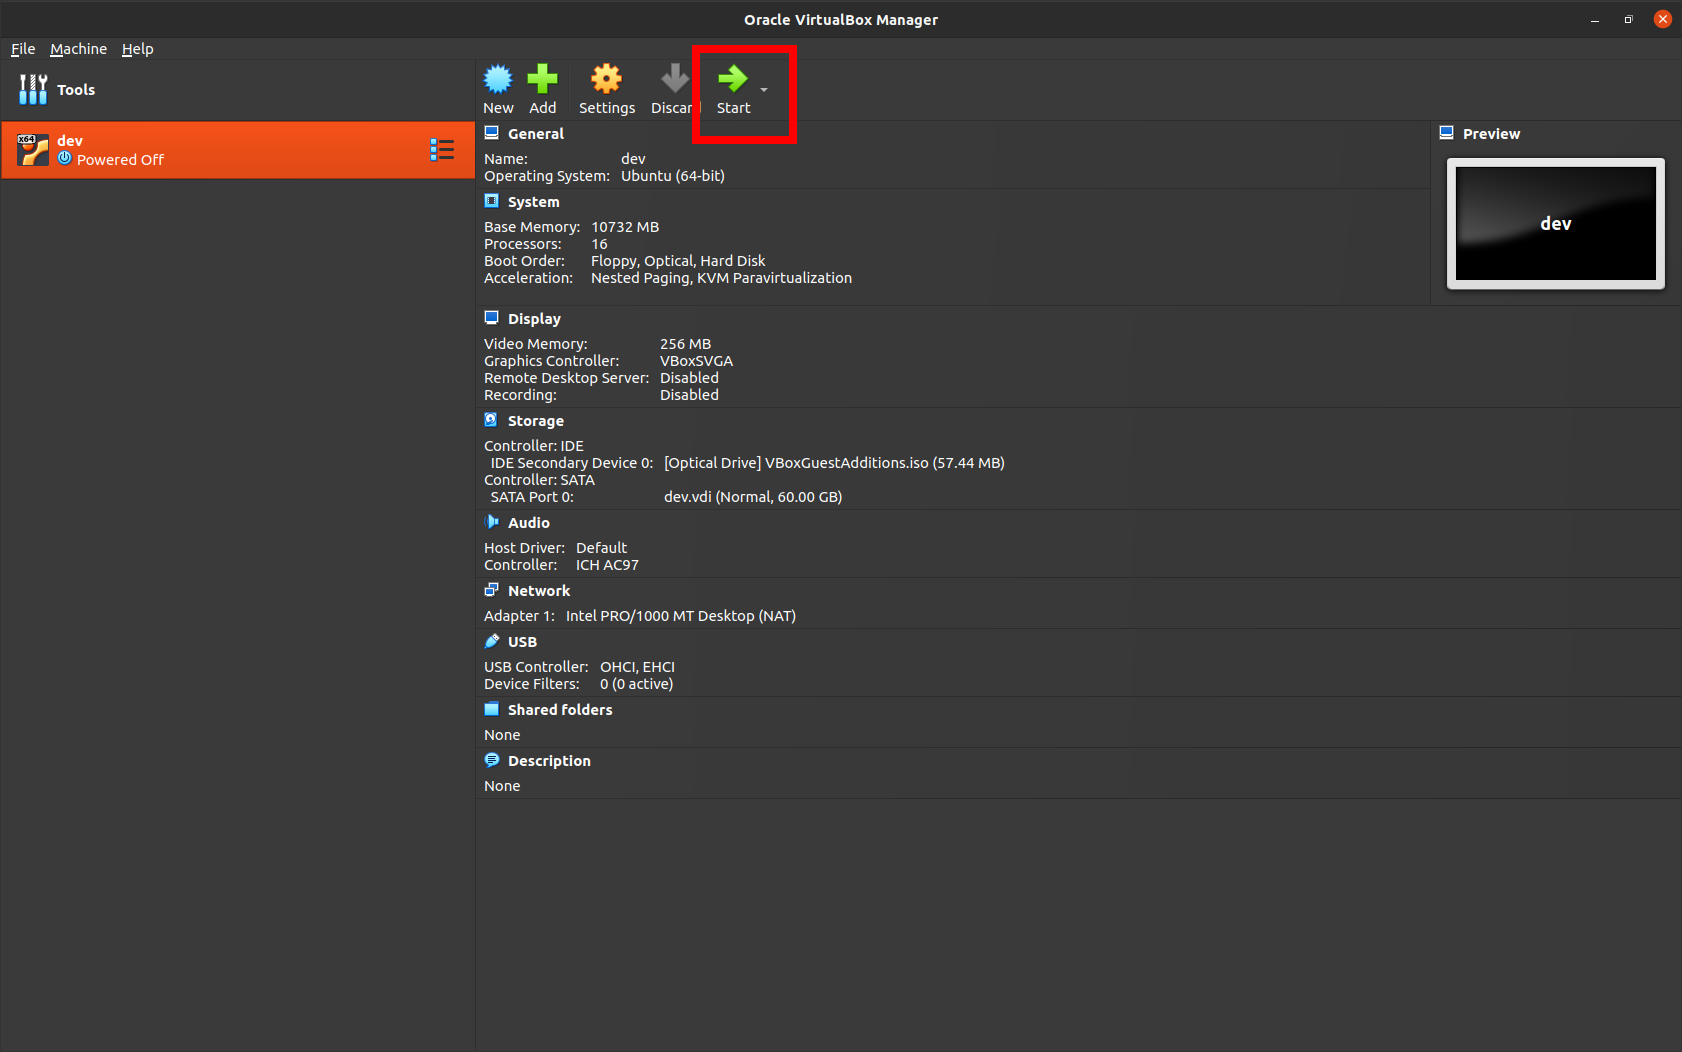
\includegraphics[width=1.0\textwidth]{Figures/vm_launch.png}
    \caption{Virtual Box main window}
    \label{fig:main_window}
\end{figure}
This will launch a new virtual box window where the system is running Ubuntu 20.04. The login the details are as follows:
\begin{itemize}
    \item \textit{User name}: dev
    \item \textit{Password}: thws
\end{itemize}

\noindent Arena-rosnav and Visual Studio Code are fully installed in this virtaul machine and are can be used now.




% Main appendix title
\chapter{Implementation Details of Social Layer Integration in Arena-Rosnav}

\label{AppendixA} % For referencing this appendix elsewhere, use \ref{AppendixA}

\label{appendix:social_layer}

This appendix documents the step-by-step procedure for integrating the social navigation layer into the costmap 
using the Arena-Rosnav simulation framework. The configuration enables socially-aware robot navigation by 
leveraging proxemic behavior modeling.

%----------------------------------------------------------------------------------------
%	SECTION 2
%----------------------------------------------------------------------------------------
\section{Repository Setup}
%-----------------------------------
%	SUBSECTION 1
%-----------------------------------
\subsection*{Step 1: Clone the \texttt{people} repository}

Clone the \href{https://github.com/DLu/people/tree/noetic}{\texttt{people}} repository into the utilities folder:

\begin{lstlisting}[language=bash]
    cd ~/arena_ws/src/arena/utils
    git clone -b noetic https://github.com/DLu/people.git
\end{lstlisting}

This repository provides the \texttt{people\_msgs} message type which must be published on the \texttt{/people} 
topic. For documentation, see: \url{https://docs.ros.org/en/api/people_msgs/html/msg/People.html}.


%-----------------------------------
%	SUBSECTION 2
%-----------------------------------

\subsection*{Step 2: Clone the \texttt{navigation\_layers} repository}

Clone the \href{https://github.com/DLu/navigation_layers/tree/noetic}{\texttt{navigation\_layers}} repository:

\begin{lstlisting}[language=bash]
    cd ~/arena_ws/src/arena/utils/navigation
    git clone -b noetic https://github.com/DLu/navigation_layers.git
\end{lstlisting}

This repository provides the \texttt{social\_navigation\_layers} package, which includes the Proxemic and Passing layers. 
See documentation: \url{http://wiki.ros.org/social_navigation_layers}.


%----------------------------------------------------------------------------------------
%	SECTION 2
%----------------------------------------------------------------------------------------
\section{Publishing \texttt{people\_msgs} from Pedsim}
%-----------------------------------
%	SUBSECTION 
%-----------------------------------
\subsection*{Step 3: Modify the \texttt{pedsim\_simulator}}

Find the simulator:

\begin{lstlisting}[language=bash]
    rospack find pedsim_simulator
\end{lstlisting}

Modify the following files to publish \texttt{people\_msgs}:
\begin{itemize}
  \item \texttt{src/simulator.cpp}
  \item Corresponding header file
\end{itemize}

Ensure the message is published on the \texttt{/people} topic.



%----------------------------------------------------------------------------------------
%	SECTION 2
%----------------------------------------------------------------------------------------
\section{Rebuild Workspace}
%-----------------------------------
%	SUBSECTION 
%-----------------------------------
\subsection*{Step 4: Rebuild with \texttt{catkin build}}

\begin{lstlisting}[language=bash]
    cd ~/arena_ws
    catkin build
\end{lstlisting}











%----------------------------------------------------------------------------------------
%	SECTION 2
%----------------------------------------------------------------------------------------
\section{Costmap Configuration}

\subsection*{Step 5: Add Social Layer Plugins}
%-----------------------------------
%	SUBSECTION 
%-----------------------------------
Edit the costmap parameters file for the robot (e.g., Jackal):

\texttt{/home/dev/arena\_ws/src/arena/simulation-setup/entities/robots \\
/jackal/configs/costmaps/global\_costmap\_params.yaml} \\

Add the following plugin:

\begin{lstlisting}[language=bash]
    - { name: proxemic_layer, type: 
    "social_navigation_layers::ProxemicLayer" }
\end{lstlisting}

Parameters for each layer are configured in: \texttt{costmap\_common\_params.yaml}

\section{Launching and Runtime Adjustment}
%-----------------------------------
%	SUBSECTION 
%-----------------------------------
\subsection*{Step 6: Launch the Simulation}

First, source the workspace and activate the virtual environment if needed:

\begin{lstlisting}[language=bash]
    source ~/arena_ws/devel/setup.bash
    roslaunch arena_bringup start_arena.launch
\end{lstlisting}
%-----------------------------------
%	SUBSECTION
%-----------------------------------
\subsection*{Step 7: Use \texttt{rqt\_reconfigure} for Dynamic Parameters}

Open a new terminal and run:

\begin{lstlisting}[language=bash]
    rosrun rqt_reconfigure rqt_reconfigure
\end{lstlisting}

This allows for real-time adjustment of social navigation parameters.


\chapter{Evaluation Pipeline for Arena-Rosnav}
\label{appendix:evaluation}

This appendix outlines the procedure for evaluating simulation results using the tools provided in the Arena-Rosnav framework.
%----------------------------------------------------------------------------------------
%	SECTION 4
%----------------------------------------------------------------------------------------
\section{Environment Setup}

\begin{enumerate}
  \item Open the Arena workspace in VS Code:
  
  \begin{lstlisting}[language=bash]
    cd /home/dev/arena_ws
    code .
  \end{lstlisting}

  \item Open a new terminal in VS Code: \texttt{Ctrl + Shift + \`}

  \item Activate the poetry environment:
  
  \begin{lstlisting}[language=bash]
    cd ~/arena_ws/src/arena/arena-rosnav
    poetry shell
    cd ~/arena_ws/src/arena/evaluation/arena_evaluation/
    scripts
  \end{lstlisting}
\end{enumerate}


%----------------------------------------------------------------------------------------
%	SECTION 4
%----------------------------------------------------------------------------------------
\section{Generating Evaluation Metrics}

\begin{enumerate}
  \item Suppose your recorded data is located at:
  
  \begin{quote}
    \texttt{/home/dev/arena\_ws/src/arena/evaluation/arena\_evaluation \\
    /data/25-05-03\_11-49-11/jackal}
  \end{quote}

  This directory should contain the following files:
  \begin{itemize}
    \item \texttt{episode.csv}
    \item \texttt{odom.csv}
    \item \texttt{params.yaml}
    \item \texttt{pedsim\_agents\_data.csv}
    \item \texttt{scan.csv}
    \item \texttt{start\_goal.csv}
  \end{itemize}

  \item Run the following command to compute evaluation metrics (replace path as necessary):

  \begin{lstlisting}[language=bash]
    python get_metrics /home/dev/arena_ws/src/arena/
    evaluation/arena_evaluation/data/25-05-03_11-49-11/
    jackal --pedsim
  \end{lstlisting}

  \item A new file \texttt{metrics.csv} will be generated in the data directory.
\end{enumerate}


%----------------------------------------------------------------------------------------
%	SECTION 4
%----------------------------------------------------------------------------------------
\section{Plotting Evaluation Results}

\begin{enumerate}
  \item Navigate to the \texttt{plot\_declarations} directory and create a YAML configuration file:

  \begin{lstlisting}[language=bash]
    cd ~/arena_ws/src/arena/evaluation/arena_evaluation
    /plot_declarations
    touch eval_teb_2025.yaml
  \end{lstlisting}

  \item Copy contents from \texttt{sample\_schema.yaml} into your new file:

  \begin{lstlisting}[language=bash]
    cp sample_schema.yaml eval_teb_2025.yaml
  \end{lstlisting}

  \item Edit the YAML file to match your evaluation data and desired plots.

  \item Generate plots using the following command (adjust path as necessary):

  \begin{lstlisting}[language=bash]
    python create_plots /home/dev/arena_ws/src/arena
    /evaluation/arena_evaluation/plot_declarations/
    eval_teb_2025.yaml
  \end{lstlisting}
\end{enumerate}

%\include{Appendices/AppendixC}

%----------------------------------------------------------------------------------------
%	BIBLIOGRAPHY
%----------------------------------------------------------------------------------------

\printbibliography[heading=bibintoc]

%----------------------------------------------------------------------------------------

\end{document}  
